\hypertarget{hash__fnv1_8c}{
\section{hash\_\-fnv1.c File Reference}
\label{hash__fnv1_8c}\index{hash_fnv1.c@{hash\_\-fnv1.c}}
}


\subsection{Detailed Description}
\begin{Desc}
\item[For internal use only.]
This file contains the implementation of the \hyperlink{group__dbprim__hash_ga7}{hash\_\-fnv1()} function, a generic hash function callback implementing the FNV-1 hash algorithm.\end{Desc}


Definition in file \hyperlink{hash__fnv1_8c-source}{hash\_\-fnv1.c}.

{\tt \#include \char`\"{}dbprim.h\char`\"{}}\par
{\tt \#include \char`\"{}dbprim\_\-int.h\char`\"{}}\par


Include dependency graph for hash\_\-fnv1.c:\begin{figure}[H]
\begin{center}
\leavevmode
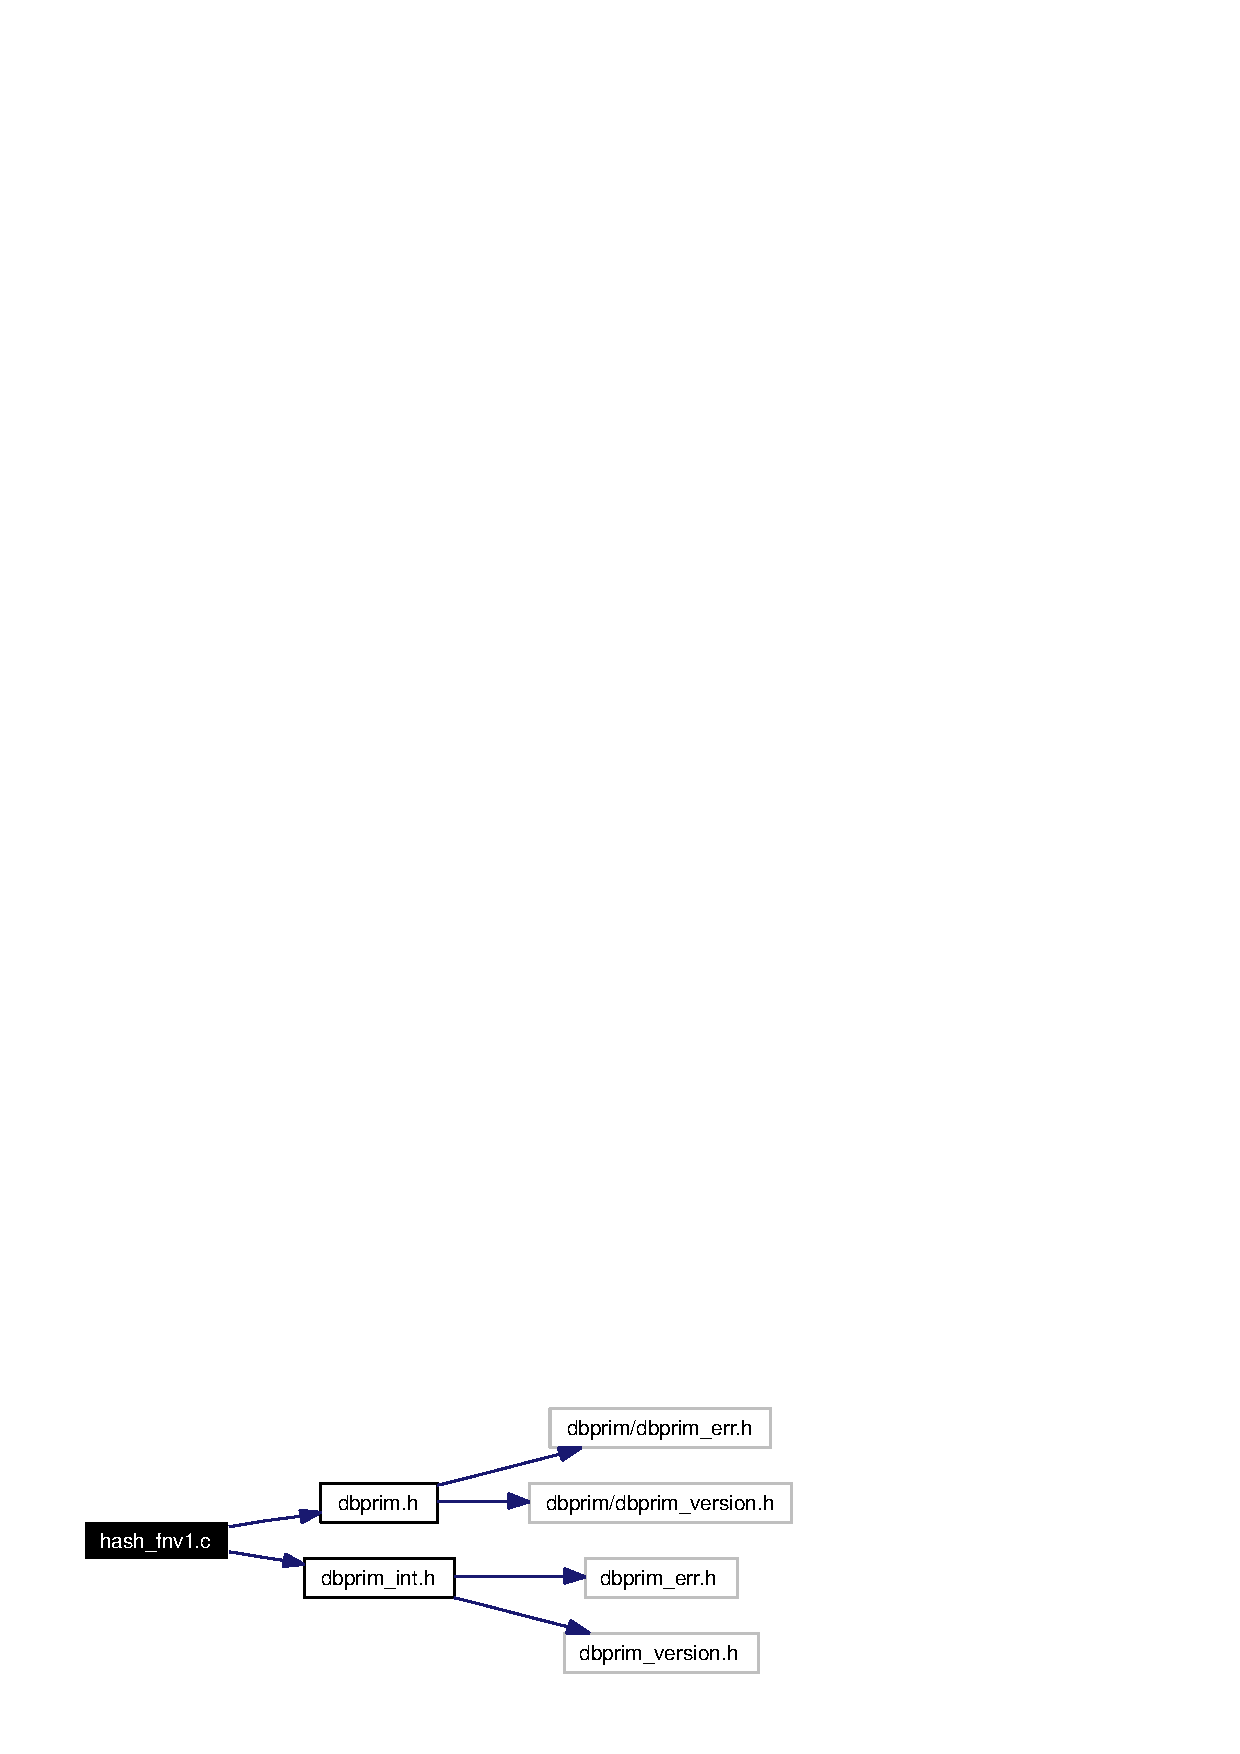
\includegraphics[width=192pt]{hash__fnv1_8c__incl}
\end{center}
\end{figure}
\subsection*{Functions}
\begin{CompactItemize}
\item 
unsigned long \hyperlink{group__dbprim__hash_ga7}{hash\_\-fnv1} (\hyperlink{struct__hash__table__s}{hash\_\-table\_\-t} $\ast$table, \hyperlink{struct__db__key__s}{db\_\-key\_\-t} $\ast$key)
\begin{CompactList}\small\item\em FNV-1 hash function. \item\end{CompactList}\end{CompactItemize}
